% !TeX root = ../../Book3.tex
% 纲要标题：### 19.2 极小图与局部模型
% 纲要位置：几何学计划纲要.md，第 2872 行。
% 正文状态：初稿；尚未正式审核。

% 纲要内容开始
% 
% * 面积积分及 Euler–Lagrange 方程
% * 一致椭圆性的梯度条件
% * 平面、悬链面及螺旋面
% * 共形参数与局部 Weierstrass 表示
% 
% 纲要内容结束

\section{极小图与局部模型}
\label{g3:sec:1902}

把超曲面写成函数的图，面积驻值就变成一个标量偏微分方程。这个方程的最高阶系数随图的斜率变化，因此一张曲面光滑并不意味着某个指定方向上的图表示始终具有统一估计。二维还有另一种参数选择：使用诱导度量的等温坐标后，极小方程化为坐标函数的调和方程，而共形条件保留为一个复代数恒等式。本节把这两种描述与三个具体模型联系起来。

\subsection{面积积分及 Euler–Lagrange 方程}
\label{g3:subsec:1902:01}
设 \(\Omega\subset\mathbb R^m\) 开，\(m\ge1\)，\(u:\Omega\to\mathbb R\) 光滑。图浸入及向上的单位法向为
\[
	F(x)=(x,u(x)),\qquad
	\nu=\frac{(-\mathrm Du,1)}{W},\qquad W=\sqrt{1+|\mathrm Du|^2}.
\]
这里 \(\mathrm D\) 是底空间的 Euclid 微分。切向量 \(F_i=(e_i,u_i)\) 给出
\begin{equation}\label{g3:eq:minimal-graph-metric}
	g_{ij}=\delta_{ij}+u_i u_j,\qquad
	g^{ij}=\delta_{ij}-\frac{u_i u_j}{W^2},\qquad
	\mu_g=W\,\mathrm dx.
\end{equation}
逆矩阵由直接相乘验证。沿 \(\mathrm Du\) 的特征值为 \(1+|\mathrm Du|^2\)，其正交补上的特征值为 \(1\)，故行列式为 \(W^2\)；在 \(\mathrm Du=0\) 处同式仍成立。因此图在一个相对紧区域 \(U\Subset\Omega\) 上的面积是
\[
	\mathcal A(u;U)=\int_U\sqrt{1+|\mathrm Du|^2}\,\mathrm dx.
\]

\begin{theorem}\label{g3:thm:minimal-graph-equation}
	设 \(m\ge1\)、\(\Omega\subset\mathbb R^m\) 开，\(u\in C^\infty(\Omega;\mathbb R)\)。其图为极小超曲面，当且仅当
	\begin{equation}\label{g3:eq:minimal-graph-divergence}
		\operatorname{div}\left(\frac{\mathrm Du}{\sqrt{1+|\mathrm Du|^2}}\right)=0.
	\end{equation}
	这也等价于图面积对全部紧支光滑竖直变分 \(u+t\varphi\) 驻值。若写平均曲率向量为 \(H=h_\nu\nu\)，其中 \(h_\nu=m^{-1}\operatorname{tr}A_\nu\)，则一般图满足
	\begin{equation}\label{g3:eq:minimal-graph-mean-curvature}
		mh_\nu=\operatorname{div}\left(\frac{\mathrm Du}{W}\right).
	\end{equation}
\end{theorem}
\begin{proof}
	令 \(\varphi\in C_c^\infty(\Omega)\)，在包含其支集的相对紧区域积分。微分积分号内的光滑函数，得到
	\[
		\left.\frac{\mathrm d}{\mathrm dt}\right|_0\mathcal A(u+t\varphi)
		=\int\frac{\mathrm Du\cdot\mathrm D\varphi}{W}\,\mathrm dx
		=-\int\varphi\operatorname{div}(\mathrm Du/W)\,\mathrm dx.
	\]
	因测试函数任意，驻值恰好给出式\eqref{g3:eq:minimal-graph-divergence}。还须核对竖直变分确实检测了全部平均曲率。按本卷 \(B=(\overline\nabla\mathrm dF)^\perp\)、\(A_\nu=-\overline\nabla\nu\) 的约定，
	\[
		h_{ij}=\langle F_{ij},\nu\rangle=\frac{u_{ij}}W,
		\qquad
		mh_\nu=g^{ij}h_{ij}
		=\frac1W\left(\delta_{ij}-\frac{u_i u_j}{W^2}\right)u_{ij}.
	\]
	展开散度恰得右端，所以式\eqref{g3:eq:minimal-graph-mean-curvature}成立。也可以从面积第一变分核对：竖直速度 \(\varphi e_{m+1}\) 的法向分量为 \((\varphi/W)\nu\)，乘面积密度 \(W\) 后，第一变分就是 \(-m\int h_\nu\varphi\,\mathrm dx\)。因 \(W>0\)，这些法向分量能检测任意紧支法向速度。
\end{proof}

二维时，清除分母后，方程写成
\begin{equation}\label{g3:eq:minimal-graph-two-dimensional}
	(1+u_y^2)u_{xx}-2u_xu_yu_{xy}+(1+u_x^2)u_{yy}=0.
\end{equation}
当 \(m=1\) 时，它给出 \(u''=0\)，所以极小曲线的图恰为直线。对 \(m\ge2\)，非线性来自不同方向的斜率相互耦合；不能把方程简单替换为 \(\sum_i u_{ii}=0\)。
\ProseParagraphBreak
高余维图也有面积方程，但属于系统。若 \(u:\Omega\to\mathbb R^q\)，令
\(G_{ij}=\delta_{ij}+\sum_\alpha u_i^\alpha u_j^\alpha\)，对行列式求导给出
\[
	\left.\frac{\mathrm d}{\mathrm dt}\right|_0\sqrt{\det G(u+t\varphi)}
	=\sqrt{\det G}\,G^{ij}\sum_\alpha u_i^\alpha\partial_j\varphi^\alpha.
\]
因此全部竖直变分的驻值方程为
\[
	\partial_i\left(\sqrt{\det G}\,G^{ij}\partial_j u^\alpha\right)=0,
	\qquad1\le\alpha\le q.
\]
它们仍等价于平均曲率向量为零：若一个法向量与全部竖直方向正交，它就是水平向量；再与各 \(F_i\) 正交就使其所有水平分量为零。下文的标量椭圆性与凸性论证固定 \(q=1\)，不会把系统中的所有非线性都归为同一个标量系数。

\subsection{一致椭圆性的梯度条件}
\label{g3:subsec:1902:02}
极小图方程的每一点都有正定主部，但其最小特征值依赖 \(|\mathrm Du|\)。先把这个依赖精确写出，才能判断\chapref{g3:ch:12}的估计何时具有统一常数。

\begin{proposition}\label{g3:prop:minimal-graph-ellipticity}
	设 \(m\ge1\)、\(\Omega\subset\mathbb R^m\) 开，\(u\in C^\infty(\Omega)\)。令
	\[
		a^{ij}(p)=\frac{\delta_{ij}}{\sqrt{1+|p|^2}}
		-\frac{p_i p_j}{(1+|p|^2)^{3/2}}.
	\]
	则图方程是 \(a^{ij}(\mathrm Du)u_{ij}=0\)，其线性化为
	\begin{equation}\label{g3:eq:minimal-graph-linearization}
		\mathcal L_u\varphi
		=\partial_i\bigl(a^{ij}(\mathrm Du)\partial_j\varphi\bigr).
	\end{equation}
	若 \(|\mathrm Du|\le L\)，则对所有 \(\xi\in\mathbb R^m\) 有
	\begin{equation}\label{g3:eq:minimal-graph-elliptic-bounds}
		(1+L^2)^{-3/2}|\xi|^2
		\le a^{ij}(\mathrm Du)\xi_i\xi_j\le|\xi|^2.
	\end{equation}
	将原方程乘以 \(W\) 后，主矩阵变成
	\(b^{ij}=\delta_{ij}-u_i u_j/W^2\)，其特征值在
	\([(1+L^2)^{-1},1]\) 内。
\end{proposition}
\begin{proof}
	对 \(p\mapsto p/\sqrt{1+|p|^2}\) 求导就是矩阵 \(a\)，再按链式法则分别对空间变量和变分参数求导，得到方程及线性化。若 \(p\ne0\)，把 \(\xi\) 分为平行于 \(p\) 与垂直于 \(p\) 的两部分，则
	\[
		a(p)\xi\cdot\xi
		=(1+|p|^2)^{-3/2}|\xi_\parallel|^2
		+(1+|p|^2)^{-1/2}|\xi_\perp|^2.
	\]
	这给出两个特征值和所述界；\(p=0\) 时 \(a=I\)。乘以 \(W\) 后两个特征值分别为 \(W^{-2}\) 和 \(1\)。
\end{proof}

\(\mathcal L_u\) 按散度形式书写，因而它在紧支测试下的二次型为负；这与本卷非负 Laplace 的记号并不矛盾。竖直变分的面积二阶导数是
\[
	\left.\frac{\mathrm d^2}{\mathrm dt^2}\right|_0\mathcal A(u+t\varphi)
	=\int a^{ij}(\mathrm Du)\partial_i\varphi\partial_j\varphi\,\mathrm dx.
\]
这个表达式在固定图坐标中为正。换成法向速度后，内在 Jacobi 二次型会出现第二基本形式的负势；两者使用不同的速度函数，不能只比较外观中的正负号。
\ProseParagraphBreak
梯度界给出统一椭圆下界，但把一族方程代入高阶内估计时，还要控制相应系数的连续模或 Hölder 范数。\Cref{g3:thm:local-elliptic-lp-apriori,g3:thm:interior-schauder}分别列出了这些要求。这里只有光滑图，局部系数都是光滑的；仅凭一个梯度上界而直接宣称任意阶常数已受控，会跳过非线性正则性中的实质步骤。
\ProseParagraphBreak
斜率发散可以来自图方向退化，而非曲面本身出现奇点。例如下一小节的悬链面上半部写成
\[
	u(x,y)=a\operatorname{arcosh}\left(\frac{\sqrt{x^2+y^2}}a\right),
	\qquad \sqrt{x^2+y^2}>a,
\]
其径向导数为 \(a/\sqrt{r^2-a^2}\)，在颈圈附近趋于无穷。悬链面在颈圈却仍是光滑浸入；失效的是向水平平面的图表示。

\subsection{平面、悬链面及螺旋面}
\label{g3:subsec:1902:03}
平面、悬链面和螺旋面分别展示零曲率、带颈圈的旋转曲面以及沿轴不断旋转的曲面。以下直接求导，既核对极小性，也给出后面稳定性计算所需的度量与曲率。

\begin{example}\label{g3:exm:minimal-plane-catenoid-helicoid}
	仿射图 \(u(x)=b\cdot x+c\) 满足 \(\mathrm D^2u=0\)，所以是极小图，且第二基本形式为零。

	对 \(a>0\)，悬链面的参数取为
	\begin{equation}\label{g3:eq:catenoid-conformal-model}
		C_a(v,\theta)
		=a(\cosh v\cos\theta,\cosh v\sin\theta,v),
		\qquad(v,\theta)\in\mathbb R\times\mathbb R/(2\pi\mathbb Z).
	\end{equation}
	一阶导数相互正交且平方长度都为 \(a^2\cosh^2v\)。取
	\[
		\nu_C=(-\operatorname{sech}v\cos\theta,
		-\operatorname{sech}v\sin\theta,\tanh v),
	\]
	它等于 \((C_v\times C_\theta)/|C_v\times C_\theta|\)。二阶导数与法向的配对依次为
	\[
		\langle C_{vv},\nu_C\rangle=-a,\qquad
		\langle C_{v\theta},\nu_C\rangle=0,\qquad
		\langle C_{\theta\theta},\nu_C\rangle=a.
	\]
	因此
	\begin{equation}\label{g3:eq:catenoid-curvature-model}
		\begin{aligned}
		g_C&=a^2\cosh^2v(\mathrm dv^2+\mathrm d\theta^2),\\
		k_1&=-\frac1{a\cosh^2v},\qquad k_2=\frac1{a\cosh^2v},\\
		K&=-\frac1{a^2\cosh^4v},\qquad |A|^2=\frac2{a^2\cosh^4v}.
		\end{aligned}
	\end{equation}
	两个主曲率的平均值为零，所以悬链面极小。第一卷第8.5.1小节用母线弧长 \(s\) 写出同一曲面；换元 \(s=a\sinh v\) 恰好给出这里的共形参数。
	% 跨卷依赖：g1:exm:catenoid-curvatures；g1:prop:revolution-two-forms。

	螺旋面可以取参数
	\begin{equation}\label{g3:eq:helicoid-model}
		T_a(s,\theta)=(s\cos\theta,s\sin\theta,a\theta),
		\qquad(s,\theta)\in\mathbb R^2.
	\end{equation}
	令 \(w=\sqrt{a^2+s^2}\)。此时
	\[
		g_T=\mathrm ds^2+w^2\mathrm d\theta^2,\qquad
		\nu_T=w^{-1}(a\sin\theta,-a\cos\theta,s).
	\]
	直接求导得到
	\[
		h_{ss}=h_{\theta\theta}=0,\qquad h_{s\theta}=-a/w.
	\]
	因逆度量为对角矩阵，平均曲率为零，而
	\(K=\det(h_{ij})/\det(g_{ij})=-a^2/(a^2+s^2)^2\)。令 \(s=a\sinh v\)，则
	\[
		T_a(v,\theta)=a(\sinh v\cos\theta,\sinh v\sin\theta,\theta),\qquad
		g_T=a^2\cosh^2v(\mathrm dv^2+\mathrm d\theta^2).
	\]
	所以悬链面和螺旋面在这些参数小片上等距，却不是通过空间刚性运动得到的同一曲面。
\end{example}

\begin{figure}[htbp]
	\centering
	% !TeX root = ../Book3.tex
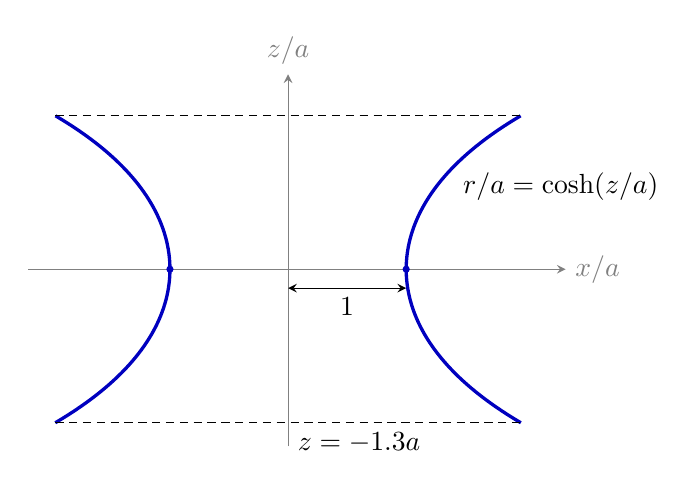
\begin{tikzpicture}[x=1.5cm,y=1.5cm,>=stealth]
	\draw[->,gray] (-2.2,0)--(2.35,0) node[right] {\(x/a\)};
	\draw[->,gray] (0,-1.5)--(0,1.65) node[above] {\(z/a\)};
	\draw[very thick,blue!75!black,domain=-1.3:1.3,samples=81]
		plot ({cosh(\x)},\x);
	\draw[very thick,blue!75!black,domain=-1.3:1.3,samples=81]
		plot ({-cosh(\x)},\x);
	\draw[densely dashed] (-1.97091,1.3)--(1.97091,1.3);
	\draw[densely dashed] (-1.97091,-1.3)--(1.97091,-1.3);
	\draw[<->] (0,-.16)--(1,-.16) node[midway,below] {\(1\)};
	\fill[blue!75!black] (1,0) circle (1.3pt);
	\fill[blue!75!black] (-1,0) circle (1.3pt);
	\node[right] at (1.4,.7) {\(r/a=\cosh(z/a)\)};
	\node[below right] at (0,-1.3) {\(z=-1.3a\)};
\end{tikzpicture}

	\caption{悬链面与过旋转轴平面的交线。将右支绕竖轴旋转得到整张曲面；颈圈半径为 \(a\)。在颈圈之外可分别写成上、下两张水平图，颈圈处则使用 \((v,\theta)\) 参数。}
	\label{g3:fig:catenoid-profile}
\end{figure}

图\ref{g3:fig:catenoid-profile}给出了悬链面的旋转轮廓。上述参数的全局性质也能直接看出。悬链面的第三坐标确定 \(v\)，前两坐标再确定 \(\theta\) 模 \(2\pi\)，故它是嵌入；紧集的原像使 \(v\) 有界，因而原像紧。螺旋面的第三坐标确定实数 \(\theta\)，前两坐标再确定 \(s\)，所以它也是适当嵌入。这里“适当”指紧集的原像为紧集，后面用它保证环境球内的参数面积有限。
\ProseParagraphBreak
两者的共形度量均不小于 \(a^2(\mathrm dv^2+\mathrm d\theta^2)\)。若一列点关于诱导距离为 Cauchy 列，则它关于平坦圆柱或平面距离也为 Cauchy 列，因而收敛；在极限附近两个光滑度量局部等价，遂也按诱导距离收敛。这证明两曲面完备。螺旋面的 \(\theta\) 不能模 \(2\pi\) 取商，否则第三坐标改变 \(2\pi a\)；这正是局部等距不能自动变成整体同一参数空间的原因。

\subsection{共形参数与局部 Weierstrass 表示}
\label{g3:subsec:1902:04}
对一般光滑极小浸入曲面，先在诱导度量上使用\cref{g3:lem:surface-isothermal-coordinate}，即可选择局部共形坐标。\Cref{g3:prop:conformal-harmonic-minimal}随后把极小性识别为三个坐标函数的调和性。Weierstrass 表示将这个描述进一步改写成全纯数据。\footnote{Karl Theodor Wilhelm Weierstrass（1815--1897），德国数学家，研究复函数、幂级数、椭圆函数与变分法。}

\begin{theorem}[局部 Weierstrass 表示]\label{g3:thm:local-weierstrass-representation}
	设 \(D\subset\mathbb C\) 为开圆盘，\(\phi_1,\phi_2,\phi_3\) 为全纯函数，满足
	\begin{equation}\label{g3:eq:weierstrass-null-condition}
		\phi_1^2+\phi_2^2+\phi_3^2=0,\qquad
		|\phi_1|^2+|\phi_2|^2+|\phi_3|^2>0.
	\end{equation}
	则对固定 \(z_0\in D\) 和 \(p\in\mathbb R^3\)，公式
	\begin{equation}\label{g3:eq:weierstrass-null-integral}
		F(z)=p+\operatorname{Re}\int_{z_0}^z(\phi_1,\phi_2,\phi_3)\,\mathrm d\zeta
	\end{equation}
	定义共形极小浸入，积分在 \(D\) 中与路径无关，诱导度量为
	\(\frac12\sum_\alpha|\phi_\alpha|^2|\mathrm dz|^2\)。反过来，每个到 \(\mathbb R^3\) 的光滑极小曲面浸入，在局部等温参数中均由此得到。
	在适当刚性旋转后缩小圆盘，还可写成
	\begin{equation}\label{g3:eq:weierstrass-fg-data}
		(\phi_1,\phi_2,\phi_3)
		=f(1-g^2,\ i(1+g^2),\ 2g),
	\end{equation}
	其中 \(f,g\) 全纯且 \(f\ne0\)，此时诱导度量为
	\begin{equation}\label{g3:eq:weierstrass-metric}
		g_F=|f|^2(1+|g|^2)^2|\mathrm dz|^2.
	\end{equation}
\end{theorem}
\begin{proof}
	全纯一形式 \(\phi_\alpha\,\mathrm dz\) 是闭的，因为其外微分等于 \(\partial_{\bar z}\phi_\alpha\,\mathrm d\bar z\wedge\mathrm dz=0\)。圆盘为星形，沿从 \(z_0\) 出发的线段积分即得原函数；对线段积分求导，或使用\cref{g3:lem:surface-isothermal-coordinate}证明中的径向原函数计算，得到其微分正是该一形式。因此沿任何路径的积分都等于原函数的端点差。
	写 \(\phi=(\phi_1,\phi_2,\phi_3)=a+ib\)，其中 \(a,b\) 为实向量，则
	\[
		F_x=a,\qquad F_y=-b.
	\]
	复双线性恒等式 \(\phi\cdot\phi=0\) 分别给出
	\(|a|^2=|b|^2\)、\(a\cdot b=0\)。非退化条件使两者都非零，故 \(F\) 共形浸入，且共形因子为 \(|a|^2=\frac12|\phi|^2\)。全纯原函数的实部调和，直接由 Cauchy--Riemann 方程也得到 \(F_{xx}+F_{yy}=0\)。所以\cref{g3:prop:conformal-harmonic-minimal}给出极小性。
	反过来，给极小浸入的诱导度量选等温坐标。写
	\(\phi=F_x-iF_y\)，则
	\[
		\partial_{\bar z}\phi=\tfrac12(F_{xx}+F_{yy})=0.
	\]
	共形性给出 \(\phi\cdot\phi=0\)，浸入性给出 \(\phi\ne0\)。又 \(\mathrm dF=\operatorname{Re}(\phi\,\mathrm dz)\)，故恢复积分表达式。
	最后，在中心适当选择环境正交坐标，使 \(\phi_1-i\phi_2\ne0\)；例如可将两个共形切向量分别送到正 \(x_1\) 轴和负 \(x_2\) 轴。缩小圆盘使该函数处处非零，令
	\[
		f=\frac{\phi_1-i\phi_2}{2},\qquad
		g=\frac{\phi_3}{2f}.
	\]
	零二次式给出 \((\phi_1-i\phi_2)(\phi_1+i\phi_2)=-\phi_3^2\)，于是
	\(\phi_1+i\phi_2=-2fg^2\)。解这两条线性等式便得式\eqref{g3:eq:weierstrass-fg-data}。展开平方模有
	\[
		|1-g^2|^2+|1+g^2|^2+4|g|^2=2(1+|g|^2)^2,
	\]
	代入度量公式即得式\eqref{g3:eq:weierstrass-metric}。
\end{proof}

这个局部版本不需要假定整张曲面已有单个复坐标。若在一个更大的黎曼曲面上给定三个全纯一形式 \(\Phi_\alpha\)，零二次式与非退化条件按坐标变换保持；它们定义全局单值映射的充要条件是
\begin{equation}\label{g3:eq:weierstrass-real-period}
	\operatorname{Re}\int_\gamma(\Phi_1,\Phi_2,\Phi_3)=0
	\quad\text{对每条分段光滑闭路 }\gamma.
\end{equation}
必要性来自对 \(\mathrm dF\) 积分；充分性来自两条端点相同的路径拼成闭路，实部积分因而相同。非零的纯虚周期可以允许，要求复周期本身全为零则过强。
\ProseParagraphBreak
公式中的 \(g\) 也可以是亚纯函数，但须先保证三个一形式实际全纯。在式\eqref{g3:eq:weierstrass-fg-data}中，若 \(g\) 在一点有 \(k\) 阶极点，\(f\) 必须至少有 \(2k\) 阶零点才能消去全部极点；恰为 \(2k\) 阶时至少一个分量在该点非零，仍为浸入。若三个全纯分量同时消失，而并非全部恒零，取最小消失阶 \(\ell\ge1\)，可写 \(\phi=(z-z_*)^\ell\psi\)、\(\psi(z_*)\ne0\)。幂级数的零点性质见第四卷第1.1.3小节。于是
\[
	g_F=\tfrac12|z-z_*|^{2\ell}|\psi(z)|^2|\mathrm dz|^2.
\]
映射仍光滑、调和且弱共形，\(z_*\) 是微分消失 \(\ell\) 阶的孤立分支点；在那里没有正定诱导度量。这项结论来自当前 Euclid 目标的全纯表示，不能无条件移到任意目标的弱共形映射。
% 跨卷依赖：g4:prop:0101:zero-order；g4:thm:0101:identity。
\ProseParagraphBreak
最后，\(f=1\)、\(g=z\) 给出
\[
	F(z)=\operatorname{Re}(z-z^3/3,\ i(z+z^3/3),\ z^2),
\]
度量为 \((1+|z|^2)^2|\mathrm dz|^2\)，与\cref{g3:ex:enneper-branched-parametrization}的直接计算一致。全纯数据保证局部浸入和极小性；它本身不保证整体单射、适当性或完备性，这些性质仍须逐个模型核对。
% 纲要条目排为编号小节标题，并进入目录与书签；说明段仍保留于纲要注释中。
